\documentclass[a4paper,10pt]{article}
\usepackage[utf8]{inputenc}
\usepackage{graphicx}
\usepackage{amsmath}
\usepackage{gensymb}
%opening
\title{Kepler's Laws and Newton's Universal Gravitation}
\author{DeepSeek \& Francesco Lazzarotto}

\begin{document}

\maketitle

\begin{abstract}
We will show a comprehensive physics lesson covering Kepler's three laws and Newton's law of universal gravitation, including how they interconnect. There will be shown examples and computations, so the response needs to be educational yet practical.
All will be structured logically: start with Kepler's laws, explaining each with clear examples and calculations, then introduce Newton's law, and finally show how Newton's law mathematically validates Kepler's laws.\\
For Kepler's first law, will be used an elliptical orbit example with aphelion and perihelion distances. For the second law, a comparative area calculation would work. The third law needs a simple ratio example. Newton's law should derive gravity's role, then link back to Kepler's third law with a clear mathematical proof.\\
The challenge is balancing depth with accessibility, keeping the math clear without oversimplifying the physics. We'll use concrete numbers (like Earth-Sun distances) to make it relatable.
\end{abstract}
\clearpage

\section{Part 1: Kepler's Three Laws of Planetary Motion}

In the early 1600s, Johannes Kepler analyzed the precise astronomical observations of Tycho Brahe. He discovered three empirical laws that described planetary motion with remarkable accuracy, moving away from the ancient idea of perfect circular orbits.

\subsection{Kepler's First Law (The Law of Ellipses):}
\begin{quote}
The orbit of a planet is an ellipse with the Sun at one focus.
\end{quote}
\begin{itemize}
\item \emph{Key Concept:} An ellipse is an oval shape with two focal points (foci). The Sun is not at the center but at one of these foci. The degree of "oval-ness" is measured by eccentricity (\emph{e}). A circle has e=0; most planetary orbits are nearly circular (e.g., Earth's e \(\approx 0.0167\)).
\end{itemize}

\subsection{Kepler's Second Law (The Law of Equal Areas):}
\begin{quote}
 A line segment joining a planet and the Sun sweeps out equal areas during equal intervals of time.
\end{quote}
\begin{itemize}
\item \emph{Key Concept:} A planet moves faster when it is closer to the Sun (perihelion) and slower when it is farther away (aphelion).
The rate at which it "sweeps out area" is constant.
\end{itemize}
\begin{figure}[!ht]
\begin{center}
 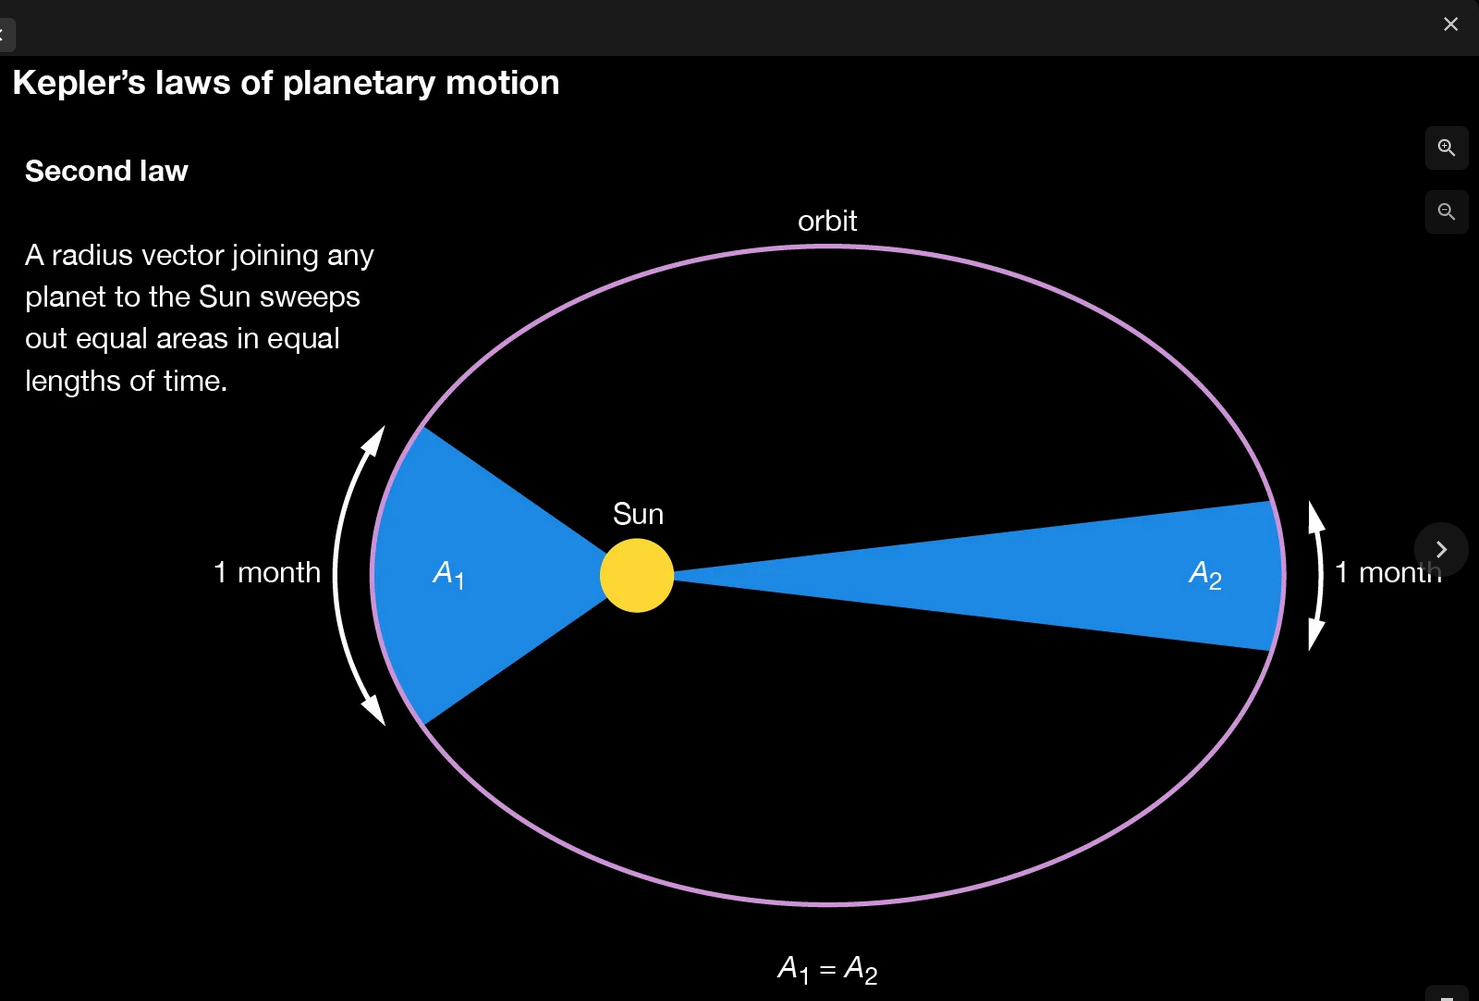
\includegraphics[width=15cm]{Kepler2ndLow.png}
\end{center}
\caption{Kepler 2nd law}
\end{figure}
Kepler’s Second Law, also known as the Law of Equal Areas, describes the speed at which a planet travels as it orbits the Sun. While the First Law defines the \emph{shape} of the orbit (an ellipse), the Second Law explains the \emph{rhythm} of planetary motion.
Kepler’s Second Law (The Law of Equal Areas).\\
In simpler terms, a planet does not move at a constant speed. Its orbital velocity changes depending on how far it is from the Sun.\\
Because orbits are elliptical and the Sun sits at one focus, the distance between the planet and the Sun is constantly changing. To ensure the "area" swept by the imaginary line stays the same, the planet must adjust its speed:
\begin{itemize}
\item At Perihelion (closest to the Sun): The "radius" line is short. To cover a specific area, the planet must travel a longer distance along its orbital path. Therefore, the planet moves at its maximum velocity.
\item At Aphelion (farthest from the Sun): The "radius" line is very long. Only a small movement along the orbit is needed to sweep out the same area. Therefore, the planet moves at its minimum velocity.
\end{itemize}
\begin{table}[h!]
\begin{center}
\begin{tabular}{|c|c|c|}
\hline
\textbf{Position}&\textbf{Distance from Sun}&\textbf{Orbital Speed}\\
\hline
Perihelion&Minimum&Fastest\\
\hline
Aphelion&Maximum&Slowest\\
\hline
\end{tabular}
\end{center}
\end{table}
\emph{The Physics Behind the Law}\\
Kepler derived this law through meticulous observation of planetary data (specifically from Tycho Brahe). However, we now understand that this is a direct consequence of the Conservation of Angular Momentum.
In a system where the only force (gravity) acts along the line connecting the two objects, the angular momentum \emph{L}
remains constant:
\[
 L = m \cdot r \cdot v \cdot \sin(\theta)
\]
Where:
\begin{itemize}
\item  m  is the mass of the planet.
\item  r  is the distance from the Sun.
\item  v  is the orbital velocity.
 \item \(\theta\)  is the angle between the radius vector and the velocity vector.
\end{itemize}
\emph{Historical Significance}\\
This law was revolutionary because it shattered the ancient Greek ideal that celestial bodies must move in "perfect" uniform circles at constant speeds. It provided the empirical groundwork for Isaac Newton to later formulate his Law of Universal Gravitation.
\subsection{Kepler's Third Law (The Harmonic Law):}
\begin{quote}
The square of the orbital period (\emph{T}) of a planet is directly proportional to the cube of the semi-major axis (\emph{a}) of its orbit.
\end{quote}
\emph{Formula:} \( T^2 \propto a^3 \) or, more precisely, \( \frac{T^2}{a^3} = \text{constant} \) for all planets orbiting the same central body.\\
While the first two laws describe the motion of a single planet, the Third Law provides a universal rule that links all planets in a system.
In simpler terms, as a planet’s distance from the Sun increases, its orbital period (=the time it takes to complete one full revolution) increases significantly.
\begin{itemize}
\item \emph{Key Concept:} This law provides a precise relationship between a planet's distance from the Sun and the time it takes to complete one orbit. The farther a planet is, the longer its year.
\end{itemize}
When expressed using Earth-based units —years for the orbital period (P) and Astronomical Units (AU) for the semi-major axis (a)— the relationship is remarkably simple:
\[
 P^2 = a^3
\]
\begin{table}[h!]
\begin{center}
\begin{tabular}{|c|c|c|c|c|}
\hline
\textbf{Planet}& \textbf{Distance (in AU)}& \textbf{Period (in Earth Years)}& \(P^2\) & \(a^3\)\\
\hline
Mercury&0.39&0.24&\(\sim0.06\)&\(\sim0.06\)\\
\hline
Earth&1.00&1.00&1.00&1.00\\
\hline
Mars&1.52&1.88&\(\sim3.53\)&\(\sim3.51\)\\
\hline
Jupiter&5.20&11.86&\(\sim141\)&\(\sim141\)\\
\hline
\end{tabular}
\end{center}
\end{table}
Note: 1 AU is the average distance from the Earth to the Sun. \\
\subsubsection{Dynamics: Distance vs. Speed}
The "Harmonic" nature of this law reveals two critical facts about our solar system:
\begin{itemize}
\item Longer Paths: Outer planets have much larger orbits to travel than inner planets.
\item Slower Speeds: Outer planets actually move at slower orbital speeds because the Sun's gravitational pull is weaker at greater distances.
\end{itemize}
This is why Mercury zips around the Sun in just 88 days, while distant Neptune takes about 165 years to complete a single orbit.
\subsubsection{Why is it called the "Harmonic" Law?}
Kepler published this law in 1619 in his work Harmonices Mundi (The Harmony of the World). He believed the universe followed a divine mathematical order similar to musical harmony. He even attempted to express the varying speeds of planets as musical scales, viewing the solar system as a "celestial choir".
\subsubsection{Modern Significance}
Beyond planetary motion, this law is a fundamental tool in modern astronomy:
\begin{itemize}
\item Calculating Mass: It allows scientists to determine the mass of stars, planets, and even the Milky Way Galaxy by observing the orbits of their satellites.
\item Exoplanet Discovery: By measuring the time it takes an exoplanet to orbit its star, astronomers can calculate exactly how far away it is and whether it sits in the "habitable zone".
\item Satellite Placement: It is used to calculate the necessary altitude for artificial satellites, such as geostationary communication satellites, to stay in a fixed position above Earth.
\end{itemize}
\subsection{Example 1: Applying Kepler's Third Law}
\emph{Problem:} Mars has an orbital period of about 1.88 Earth-years. The semi-major axis of Earth's orbit is 1 Astronomical Unit (AU). What is the semi-major axis of Mars' orbit in AU?\\
\emph{Solution:}\\
Using Kepler's Third Law, \( \frac{T^2}{a^3} \) is constant for all planets orbiting the Sun. We can set up a ratio using Earth's values as a reference.\\
For Earth: \( T_{earth} = 1 \, \text{year} \), \( a_{earth} = 1 \, \text{AU} \)\\
For Mars: \( T_{mars} = 1.88 \, \text{years} \), \( a_{mars} = ? \)\\

\[
\frac{T_{earth}^2}{a_{earth}^3} = \frac{T_{mars}^2}{a_{mars}^3}
\]
\[
\frac{1^2}{1^3} = \frac{(1.88)^2}{a_{mars}^3}
\]
\[
1 = \frac{3.5344}{a_{mars}^3}
\]
\[
a_{mars}^3 = 3.5344
\]
\[
a_{mars} = \sqrt[3]{3.5344} \approx 1.52 \, \text{AU}
\]

\emph{Answer:} Mars is, on average, 1.52 times farther from the Sun than Earth is.\\

\section{Part 2: Newton's Law of Universal Gravitation}

About 50 years after Kepler, Isaac Newton formulated his law of universal gravitation, which explains \emph{why} Kepler's laws work.

\begin{quote}
Every particle in the universe attracts every other particle with a force that is directly proportional to the product of their masses and inversely proportional to the square of the distance between their centers.                                                                                                                                                                                                                      \end{quote}
\emph{Formula:} \( F = G \frac{m_1 m_2}{r^2} \)\\
\begin{itemize}
\item   \emph{F} is the gravitational force (Newtons, N)
\item   \emph{G} is the universal gravitational constant (\( 6.67430 \times 10^{-11} \, \text{N·m}^2/\text{kg}^2 \))
\item   \emph{\(m_1\)} and \(m_2\) are the masses of the two objects (kilograms, kg)
\item   \emph{r} is the distance between their centers (meters, m)
\end{itemize}

\subsection{Example 2: Calculating Gravitational Force}

\emph{Problem:} What is the gravitational force of attraction between the Earth and the Moon?\\
\begin{itemize}
\item   Mass of Earth, \( M_E = 5.97 \times 10^{24} \, \text{kg} \)
\item   Mass of Moon, \( M_M = 7.35 \times 10^{22} \, \text{kg} \)
\item   Average distance between centers, \( r = 3.84 \times 10^8 \, \text{m} \)
\end{itemize}

\emph{Solution:}\\
\[
F = G \frac{M_E M_M}{r^2}
\]
\[
F = (6.67430 \times 10^{-11}) \frac{(5.97 \times 10^{24})(7.35 \times 10^{22})}{(3.84 \times 10^8)^2}
\]
First, calculate the numerator: \( (5.97 \times 10^{24}) \times (7.35 \times 10^{22}) = 4.387 \times 10^{47} \)\\
Then the denominator: \( (3.84 \times 10^8)^2 = 1.475 \times 10^{17} \)\\
Now, \( \frac{4.387 \times 10^{47}}{1.475 \times 10^{17}} = 2.976 \times 10^{30} \)\\
Finally, \( (6.67430 \times 10^{-11}) \times (2.976 \times 10^{30}) \approx 1.98 \times 10^{20} \, \text{N} \)\\
\emph{Answer:} The gravitational force between the Earth and Moon is approximately \( 2.0 \times 10^{20} \, \text{Newtons} \).\\
This immense force is what keeps the Moon in orbit.

\section{Part 3: How are Explained Kepler's Laws}

Newton showed that his law of gravitation, when combined with his laws of motion, \emph{predicts} Kepler's empirical laws.

\subsection{Explaining Kepler's First Law (Elliptical Orbits):}
Newton demonstrated that the inverse-square nature of the gravitational force (\( F \propto 1/r^2 \)) necessarily leads to \emph{conic sections} as the possible orbits. An ellipse is one type of conic section. The other solutions (like parabolas and hyperbolas) describe the paths of objects that are not gravitationally bound, like some comets.

\subsection{Explaining Kepler's Second Law (Equal Areas):}
This is a consequence of the \emph{conservation of angular momentum}. The gravitational force is a \emph{central force}; it always acts along the line connecting the planet to the Sun. A central force exerts zero torque, meaning angular momentum must be conserved. It can be showed that constant angular momentum is mathematically equivalent to the "equal areas in equal times" rule.\\
The concept of Angular Momentum is fundamentally linked to Kepler’s Second Law, the formal discovery and enunciation of its conservation did not happen all at once. It evolved from a mathematical observation into a core principle of physics.
\subsubsection{The Mathematical Foundation: Leonhard Euler (1744)}
While Johannes Kepler described the behavior of planets (equal areas in equal times), he did not understand the underlying physics. The first person to formally describe the concept of "moment of momentum" (the precursor to angular momentum) was the Swiss mathematician Leonhard Euler.\\
In 1744, Euler began to express the idea that the "quantity of motion" for a rotating body was conserved, specifically in the context of his work on the motion of rigid bodies.
\subsubsection{The Physical Enunciation: Daniel Bernoulli (1744)}
In the same year, Daniel Bernoulli (a contemporary and friend of Euler) stated the principle more clearly in a physical sense. He realized that for a system not subject to an external torque, the total moment of momentum remains constant.
Bernoulli and Euler essentially "discovered" the principle while trying to apply Newton’s laws of motion to rotating objects—something Newton himself hadn't fully explored in his Principia.
\subsubsection{The "Law of Areas": Patrick d'Arcy (1747)}
The specific connection between Kepler’s Second Law and the conservation of angular momentum was formalized by the Irish-born mathematician Patrick d'Arcy.
\begin{itemize}
\item In 1747, he published his "Principle of Areas."
\item He explicitly stated that for any system of bodies acting on each other (under central forces), the sum of the products of the masses and the areas described by their radius vectors remains constant.
\item This was the definitive proof that Kepler's Second Law was actually the Conservation of Angular Momentum in action.
\end{itemize}
\begin{table}[h!]
\begin{center}
\begin{tabular}{|c|c|c|}
\hline
\textbf{Scientist}&\textbf{Contribution}&\textbf{Year}\\
\hline
Johannes Kepler&Observed the result (Equal Areas Law) but lacked the physics.&1609\\
\hline
Leonhard Euler&Developed the mathematical "moment of momentum."&1744\\
\hline
Patrick d'Arcy&Enunciated the "Law of Areas" as a conservation principle.&1747\\
\hline
Emmy Noether&Proved why it's conserved (due to rotational symmetry).& 1915\\
\hline
\end{tabular}
\end{center}
\caption{Key Milestone Summary}
\end{table}
\subsubsection{The "Deep" Why: Noether’s Theorem}
It is worth noting that we didn't fully understand why angular momentum is conserved until Emmy Noether published her famous theorem in 1915. She proved that every conservation law is tied to a symmetry in nature:
\begin{quote}
    \emph{Angular Momentum is conserved because space is isotropic} (it has no preferred direction).
\end{quote}
If you rotate an entire physics experiment by \(90^{\circ}\), the laws of physics don't change—and that "symmetry" is what forces angular momentum to stay constant
\subsection{Deriving Kepler's Third Law (from Newton's Law):}
This is the most powerful connection. Let's derive it for a circular orbit (a special case of an ellipse where the semi-major axis 'a' is the radius 'r').

For a planet of mass \( m \) orbiting the Sun of mass \( M_S \) at a distance \( r \), two things are true:
\begin{enumerate}
\item \emph{Newton's 2nd Law:} The gravitational force provides the centripetal force: \( G \frac{M_S m}{r^2} = m a_c \)
\item \emph{Centripetal Acceleration:} \( a_c = \frac{v^2}{r} \)
\end{enumerate}
Substituting (2) into (1):\\
\[
G \frac{M_S m}{r^2} = m \frac{v^2}{r}
\]
Cancel \( m \) and one \( r \):
\[
G \frac{M_S}{r} = v^2
\]
The orbital velocity \( v \) is the circumference (\( 2\pi r \)) divided by the period (\( T \)): \( v = \frac{2\pi r}{T} \)\\
Substitute for \( v^2 \):\\
\[
G \frac{M_S}{r} = \left( \frac{2\pi r}{T} \right)^2
\]
\[
G \frac{M_S}{r} = \frac{4\pi^2 r^2}{T^2}
\]
Now, rearrange to get \( T^2 \) on one side:\\
\[
T^2 = \frac{4\pi^2 r^2}{G M_S} \cdot r
\]
\[
T^2 = \left( \frac{4\pi^2}{G M_S} \right) r^3
\]
Since for an ellipse, we use the semi-major axis \( a \), the general form is:
\[
\boxed{T^2 = \frac{4\pi^2}{G M_S} a^3}
\]
This is Kepler's Third Law! Notice that \( \frac{4\pi^2}{G M_S} \) is a \emph{constant} because G and the mass of the Sun are constant. Therefore, \( T^2 \propto a^3 \), exactly as Kepler stated.

\section{Summary}
\begin{itemize}
\item   \emph{Kepler} described \emph{how} the planets move (kinematics).
\item   \emph{Newton} explained \emph{why} they move that way by providing the underlying force (dynamics).
\item   \emph{Newton}'s Law of Universal Gravitation is the fundamental principle that, when applied, mathematically predicts and validates all three of Kepler's Laws.
\end{itemize}
This elegant connection between observation and theory is a cornerstone of classical physics and our understanding of the cosmos.
\end{document}
